\documentclass[a4paper,11pt]{article}
\usepackage{graphicx}
\usepackage{onecolpceurws}
\usepackage{url}
\usepackage{hyperref}

\title{The TTC 2014 Movie Database Case}

\author{
Tassilo Horn\\ University of Koblenz-Landau\\ Germany\\ horn@uni-koblenz.de
\and
Christian Krause\\ SAP Innovation Center\\ Germany\\ christian.krause01@sap.com
\and
Matthias Tichy\\ Chalmers $|$ University of Gothenburg, Sweden \\matthias.tichy@cse.gu.se
}

\institution{}

\begin{document}
\maketitle

\begin{abstract}
  Social networks and other web 2.0 platforms use huge amounts of data
  to offer new services to customers. Often these data can be
  expressed as huge graphs and thus could be seen as a potential new
  application field for model transformations. However, this
  application area requires that model transformation tools scale to
  models with millions of objects. This transformation case targets
  this application area by using the IMBDB movie database as a
  model. The transformation deals with identifying all cliques of $n$
  actors which perform in the same movies.
  \end{abstract}
\vskip 32pt


\section{Introduction (MTT)}

The driving force behind social networks and other new web 2.0
offerings is often huge amount of data. Consequently, concepts like
MapReduce \cite{Dean08} and libraries like Hadoop \cite{Hadoop} and
Giraph \cite{Giraph} have been developed to efficiently process these
huge amount of data. However, model transformation approaches have so
far not adressed this field.

Automotive software is an already well-established application field
for model-driven software engineering and its models approach also
huge sizes. As a consequence from these two examples, model
transformation approaches must be scalable to models with million
objects to be applicable for these application areas.

We present in the following a case which uses the IMDB movie database
\cite{IMDBDATA} as a data source. The IMDB movie database contains
information about movies, actors performing in the movies, movie
ratings, etc. The main task is to develop a model transformation which
identifies \emph{all} cliques of $n$ actors which perform in the same
movies and calculate the average rating of those movies. Evaluation
criteria are correctness and performance.

In the following section, we describe the case in more detail
including the meta model as well as the different basic and extension
tasks. After that, Section \ref{sec-eval} presents the evaluation
criteria for submitted solutions to this case.


\section{Detailed Case Description (MTT)}\label{sec-case}

MM and data\\

The transformation is on data from a movie database.
We use the metamodel shown in Figure~\ref{fig:metamodel}.
We generate synthetic test data and also use real data
from the IMDB movie database. You can use the EMF model and
parser provided in \cite{IMDB2EMF} for this purpose.


\begin{figure}[ht]
\centering
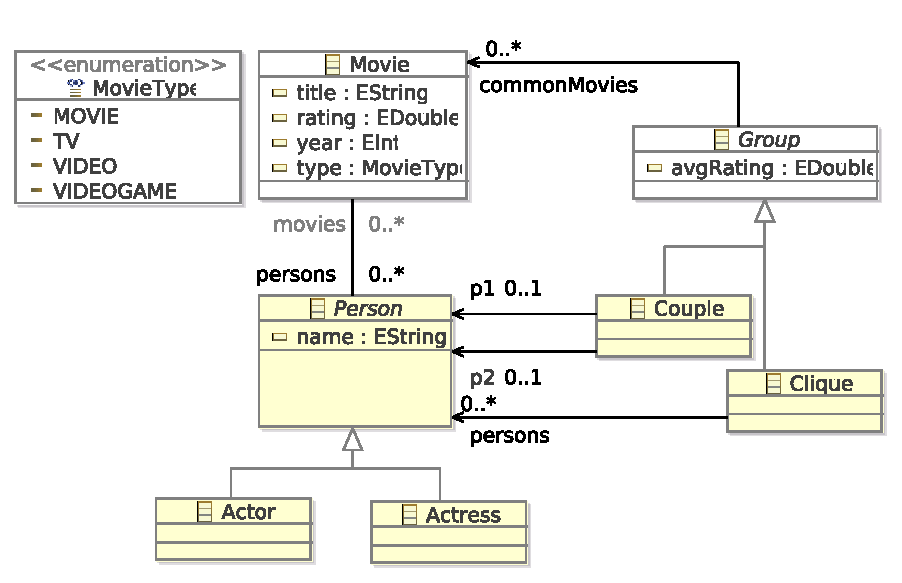
\includegraphics[width=0.6\textwidth]{movies}
\caption{Simplified metamodel for the movie database.}
\label{fig:metamodel}
\end{figure}

\subsection{Task 1: Generating Test Data (CK)}
\label{sec:gen-test-data}

The first task is to generate some test data.
This will be used to test the correctness and to do benchmarks later.
The generation of the test data should go as follows...
A graphical Henshin specification is shown in Figure~\ref{fig:gen-test-data}

\begin{figure}[p]
\centering
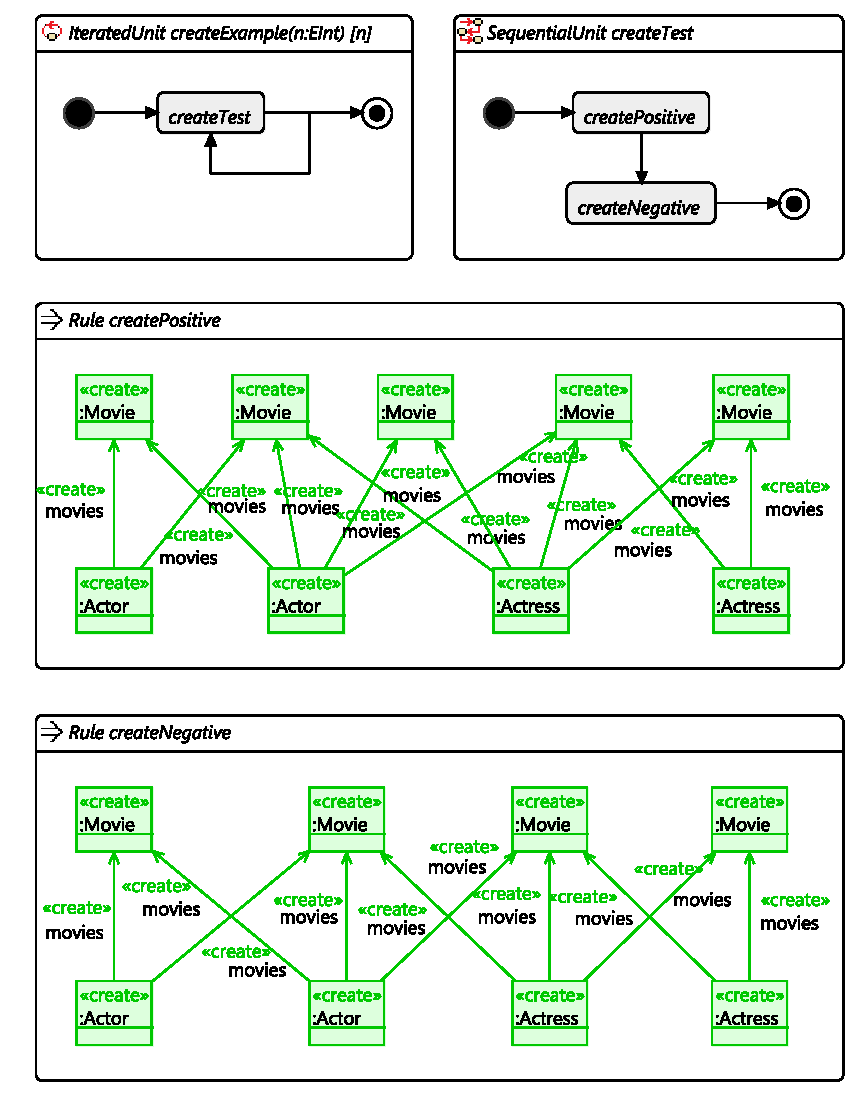
\includegraphics[width=0.8\textwidth]{gen-test-data}
\caption{Henshin specification for generating synthetic movie test data.}
\label{fig:gen-test-data}
\end{figure}

\subsection{Task 2: Finding Couples (CK)}

Implementation of the task


\subsection{Task 3: Computing Average Rankings (CK)}

Implementation of the task

\subsection{Extension Task 1: Compute Top-Ten Couples (TH)}

The goal of this task is to produce top-ten lists of the couples created by
Task~2.  For this purpose, two model queries should be given.

\begin{enumerate}
\item[(a)] Compute the top-ten couples according to the number of common movies.
\item[(b)] Compute the top-ten couples according to the average rating of their
  common movies (requires Task~3 to be solved).
\end{enumerate}

Each of the couples in the top-ten lists should be printed with the names of
the two persons, the average rating (only if Task~3 has been solved), and a
list of the couple's common movies, each movie with its title and rating.

\subsection{Extension Task 2: Finding Cliques (TH)}

This extension task is a generalization of Task~2.  A clique is a group of at
least \(n\) persons (with \(n \geq 3\)) acting together in at least 3 movies.
So a couple is essentially a clique of size \(n = 2\).

The extension task is to find cliques of a given size \(n\), and to create a
\verb|Clique| element for each of them referencing the clique's members, and
its common movies like the couples in Task~2.

The task will be evaluated for \(n \in \{3, 4, 5\}\), so it can be solved by
writing three similar rules manually.  However, to achieve a full completeness
score for this task, a solution should work for any \(n \geq 3\).  Therefore, a
transformation could have \(n\) as a parameter, or there could be a
higher-order transformation that receives \(n\) and generates a rule creating
cliques of exactly that size.

It would be interesting to be able to specify the required number of common
movies \(c\) freely.  By default and according to Task~2, \(c\) is fixed to 3.
You can earn an extra bonus point if \(c\) may be customized.


\subsection{Extension Task 3: Compute Average Rankings for Cliques (TH)}

Like it was done for couples in Task~3, the \verb|avgRating| attribute of
cliques should be set to the average rating of all its common movies.

\subsection{Extension Task 4: Compute Top Ten Cliques (TH)}

This is a variant of Extension Task~1 for cliques instead of couples.  Again,
two queries should be given.

\begin{enumerate}
\item[(a)] Compute the top-ten cliques of size \(n\) according to the number of
  common movies.
\item[(b)] Compute the top-ten cliques of size \(n\) according to the average
  rating of their common movies (requires Extension Task~3 to be solved).
\end{enumerate}

Again, every clique should be printed with the names of its members, the
average rating, and the list of common movies, each movie with its title and
rating.


\section{Evaluation Criteria (MTT)}\label{sec-eval}

Test data from December 2013. Contact us to get the data.

\subsection{Correctness Tests (TH)}

Correctness is checked using the synthetic data.

We provide: number of couples and top ten lists.

\subsection{Benchmarks (CK)}

Perform benchmarks using the following input data sets:
\begin{enumerate}
\item the synthetic data generated in Section~\ref{sec:gen-test-data}, and 
\item the IMDB data (available at \cite{IMDBDATA}; parse, e.g., using \cite{IMDB2EMF}).
\end{enumerate}
For both cases, you should run the transformation and measure 
the time needed to complete the transformation (without loading 
and saving the model).

There are two versions of the transformations: Finding Couple and Finding Cliques.
Please run the benchmarks for both versions and both data sets.

%% Tassilo: Why not measuring Task 2 on its own?

Plot the benchmarks. On the x-axis you print the size of the data set
in number of nodes and on the y-axis you plot the time. The number of nodes
includes all types of nodes (movies and persons). Make the measurements in
steps of 100,000 nodes. For the synthetic data, choose n=?,...,?
For the IMDB data, take the whole data set and to sampling. You can use
the sampler provided in \cite{IMDB2EMF}.

NOTE TO US: IMPLEMENT SAMPLING!



\bibliographystyle{plain}
\bibliography{biblio}

\appendix

\section{Expected Number of Couples and Cliques}
\label{sec:expected-numbers}

\begin{table}[h!]
  \centering
  \begin{tabular}{| l | r | r | r | r |}
  \hline
  \textbf{Model} & \textbf{\#Couples} & \textbf{\#Triples} & \textbf{\#Quadruples} & \textbf{\#Quintuples}\\
  \hline
  \hline
\end{tabular}
\caption{The synthetic models with the expected numbers of Couples and Cliques of various sizes}
\label{tab:synthetic-numbers}
\end{table}


\begin{table}[h!]
  \centering
  \begin{tabular}{| l | r | r |}
  \hline
  \textbf{Model}              & \textbf{\#Couples} & \textbf{\#Triples}\\
  \hline
  imdb-0005000-49930.movies   & 17352 & 127825\\
  imdb-0010000-98168.movies   & 28211 & 188712\\
  imdb-0030000-207420.movies  & 35198 & 200532\\
  imdb-0045000-299504.movies  & 43294 & 210985\\
  imdb-0065000-404920.movies  & 57889 & 220891\\
  imdb-0085000-499995.movies  & 79470 & 243314\\
  imdb-0105000-591042.movies  & 104479 & 276499\\
  imdb-0130000-709551.movies  & 136956 & 307405\\
  imdb-0150000-796950.movies  & 164463 & 340755\\
  imdb-0175000-901769.movies  & 208155 & 427824\\
  imdb-0200000-1004463.movies & 244627 & 457833\\
  imdb-0225000-1096479.movies & 298390 & 594032\\
  imdb-0255000-1204331.movies & 361858 & 721604\\
  imdb-0280000-1296503.movies & 408151 & 781216\\
  imdb-0310000-1402659.movies & 508839 & 1346807\\
  imdb-0340000-1505143.movies & 585689 & 1469156\\
  imdb-0370000-1603848.movies & 653715 & 1544170\\
  imdb-0400000-1702751.movies & 740961 & 1660769\\
  imdb-0430000-1793844.movies & 829136 & 1892483\\
  imdb-0465000-1904728.movies & 930509 & 2043816\\
  imdb-0495000-2000900.movies & 1017752 & 2173809\\
  imdb-0525000-2098976.movies & 1113226 & 2332100\\
  imdb-0560000-2205192.movies & 1222959 & 2525431\\
  imdb-0590000-2293503.movies & 1309101 & 2684821\\
  imdb-0625000-2397550.movies & 1441850 & 3656513\\
  imdb-0660000-2501893.movies & 1562317 & 3953798\\
  imdb-0695000-2605751.movies & 1687269 & 4253567\\
  imdb-0725000-2696312.movies & 1805982 & 4677444\\
  imdb-0760000-2800659.movies & 2034680 & 5403338\\
  imdb-0795000-2904388.movies & 2166743 & 5724736\\
  imdb-0830000-3003237.movies & 2308300 & 6148282\\
  imdb-0865000-3097577.movies & 2434934 & 6453770\\
  imdb-0900000-3193920.movies & 2558365 & 6773334\\
  imdb-all-3257145.movies     & 2709371 & 8227081\\
  \hline
\end{tabular}
\caption{The IMDb Models with the expected numbers of Couples and Triples (Cliques of size 3)}
\label{tab:imdb-numbers}
\end{table}

\section{Expected Top-Ten Lists}
\label{sec:expected-top-ten}



\end{document}


